\section{Problem Formulation}
\label{sec:problemformulation}

%\begin{table*}[t] 
\centering % centering table 
\begin{tabular}{|l|r|} % creating 12 columns 
\hline %\hline % inserting double-line 
% Entering 1st row 
$\alpha$   & Path Loss Exponent     \\
\hline % inserts single-line 
R & Communication Range \\
\hline % inserts single-line 
$I_r$ & Interference Range \\
\hline % inserts single-line 

\end{tabular} 
\label{tab:2channelcombination} 
\caption{Throughput achieved through Gateway nodes (Mbps) for various combinations of WiFi and White Space (WS) mesh topologies (Offered Load = 4 Mbps, Network Size = 30 mesh nodes).} % title name of the table 
\vspace{-0.1in}
\end{table*} 


% Organization of the Sec
In this section, we formulate the problem of how to optimally 
use WiFi and white space bands in concert when deploying wireless 
mesh networks.  We first describe our system model and illustrate 
the challenges of such a WhiteMesh architecture.  We then discuss
how to evaluate WhiteMesh networks and the corresponding goal of
both the optimization framework and the heuristic algorithms that 
we will propose in the following section.  Finally, we present 
our integer linear programming model used to address the problem. 
 
\subsection{WhiteMesh Network Architecture}
\label{subsec:architecture}

%A node in ~\emph{Multiband Wireless Mesh Network} has limited multiple slots for installing radios working in different bands. 
%Two nodes share the same link should have a common channel. The sum of the loads on the links should 
% Explain propagation, factors of the environment and so on
Wireless propagation is the behavior of the signal loss characteristics 
when wireless signals are transmitted from a transmitter to receiver.
The strength of the receiving signal depends on both the line-of-sight
path (or lack thereof) and multiple other paths that are a result of 
reflection, diffraction, and scattering from obstacles in the 
environment~\cite{andersen1995propagation}. The widely-used, Friis
equation characterizes the power of the received signal $P_r$ in terms 
of the power $P_t$ and gain $G_t$ of the transmitting signal, gain of 
the receiver $G_r$, wavelength $\lambda$ of the carrier frequency, 
distance $R$ from transmitter to receiver, and path loss exponent $n$ according 
to~\cite{friis}:
\begin{equation}
\label{eq:friis}
P_r=P_t+G_t+G_r+10n log_{10}(\frac{\lambda}{4\pi R})
\end{equation}
Here, the path loss exponent $n$ changes according to the
aforementioned environmental factors and ranges from 2 to 5 in typical
outdoor settings~\cite{rappaport}.


%The rules of radio propagation are complex and diverse,
%such as the daily changes of environment, weather, and atmosphere changes due to cosmos activities.
%In most propagation models there are three basic propagation mechanisms: reflection, diffraction, and scattering ~\cite{andersen1995propagation}.
%For multiband mesh backhual network, the nodes are usually installed on the top of buildings or towers to get the best line of sight propagation. A line of sight propagation model is a reasonable hypotheses in wireless mesh network.
% propagation fomular, explain the band influence
%In popular \emph{Friis} propagation model, the received signal power of a node is represented as:
%\begin{equation}
%\label{eq:friis}
%P_r=P_t+G_t+G_r+10n log_{10}(\frac{\lambda}{4\pi R})
%\end{equation}
%
%Path-loss exponent \emph{$n$} is used to describe the environment factors, typically in outdoor environments range from 2 to 5.\cite{camp2006measurement}.
%In equation ~\ref{eq:friis}, in the specific environment with a common path-loss exponent and $P_t,G_t,G_r$ configuration, the received signal vary according to the band represented by wavelength $\lambda$.
%Since wireless radios have the same received signal threshold, lower frequency band could have a larger communication range $D_c$, and also a larger interference range $D_r$.

% Explain multiband vs multichannel
A common assumption that use many WiFi channels is that the
propagation characteristics of one channel is similar to another, 
since the channel separation is relatively small (e.g., 22 MHz for 
the 2.4 GHz band).
Many works which rely on such an assumption have focused on the 
allocation of multiple WiFi channels with multiple radios in 
multihop wireless networks~\cite{si2010overview}.  Here, a frequency 
band is defined as a group of channels which have
similar propagation characteristics.
%We use a similar assumption for %channels within a frequency band, but consider the propagation 
%differences of a channel in one band (e.g., 450 MHz) as compared to 
%another (e.g., 2.4 GHz). 
In this work, we consider the diverse propagation characteristics
for four total frequency bands: 450 MHz, 800 MHz, 2.4 GHz, and 5.8 GHz.
The two former frequency bands, we refer to as white space (WS) bands whereas
the two latter frequency bands, we refer to as WiFi bands.

Wireless mesh networks are a particular type of multihop wireless network
that are typically considered to have at least two
tiers~\cite{CRSK06}: {\it (i)} an access tier, where client traffic 
is aggregated to and from mesh nodes, and {\it (ii)} a multihop 
backhaul tier for connecting all mesh nodes to the Internet through 
gateway nodes. In this work, we focus on how to optimally allocate 
white space and WiFi bands on a finite set of radios per mesh node
along the backhaul tier since we assume that client devices will use 
WiFi (due to the economies of scale).  In each of the WhiteMesh 
topologies studied in Section~\ref{sec:experimentdesign}, a sufficient 
number of orthogonal WiFi channels remain for the access tier to 
connect to clients using additional radios co-located on the mesh nodes.

\begin{figure}
\vspace{-0.1in}
\centering
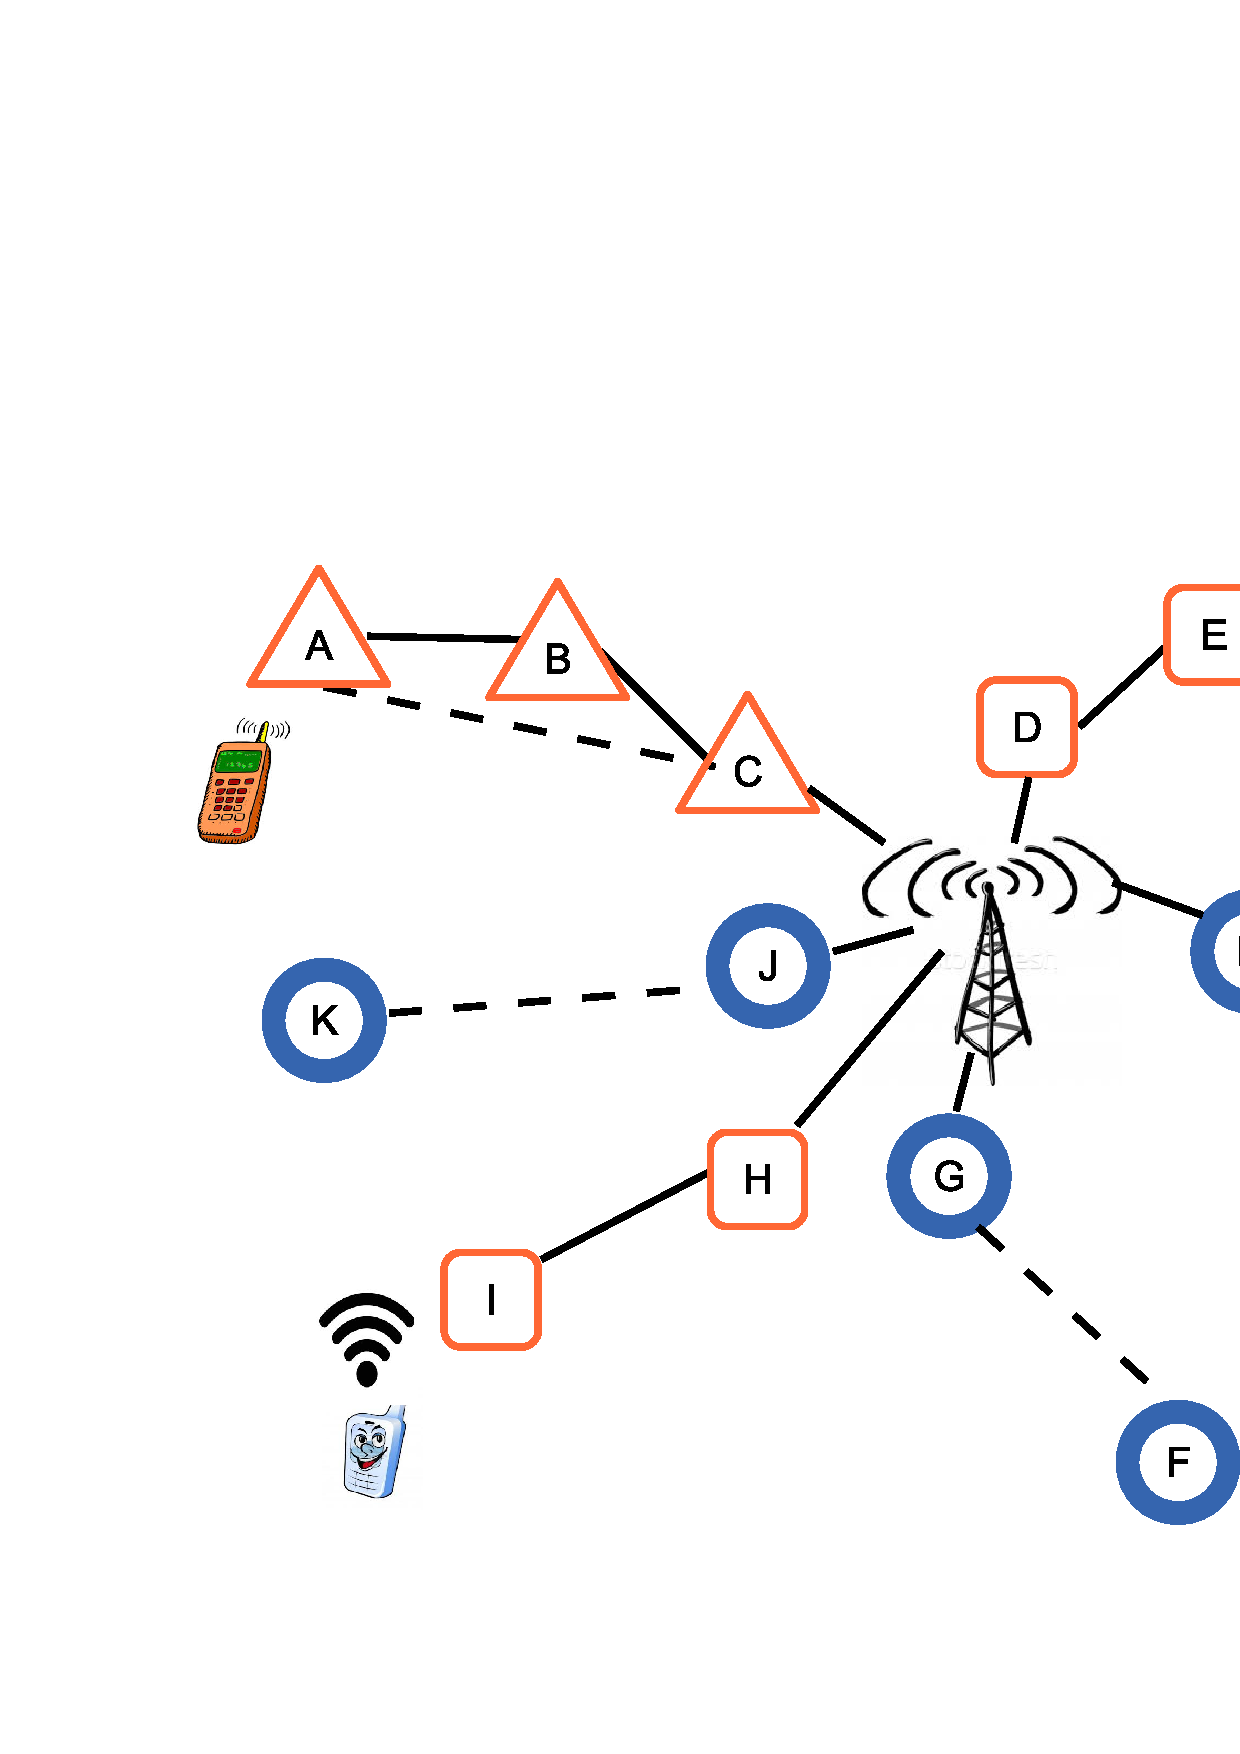
\includegraphics[width=94mm]{figures/interferencerange}
\vspace{-0.5in}
\caption{Example WhiteMesh topology with different mesh-node shapes 
representing different frequency band choices per link.}
\label{fig:interferencerange}
\vspace{-0.2in}
\end{figure}

% Make multiband challenges
Due to the broadcast nature of the wireless medium, greater levels of
propagation induce higher levels of interference.  Thus, in sparsely-populated
rural areas, the lower frequencies of the white space bands might be a
more appropriate choice for multihop paths to gateways with reduced hop
count. However, as the population and demand scales up (e.g., for more 
urban regions), the reduced spatial reuse and greater levels of interference 
of white space bands might detract from the overall deployment strategy. In 
such urban areas, select links of greater distance might be the most 
appropriate choice for white space bands, especially since the number of 
available channels is often inversely proportional to the population (due 
to the existence of greater TV channels).
%The broadcast nature of the wireless medium makes it generate multiple access interference in wireless network.
%Employing White Space Band in lower frequency brings advantages for mesh network, 1) more orthogonal bandwidth reduce the contention and conflict in the network,
% 2) the propagation variation brings flexible topology by reducing connection hop counts in the network.
%However, at the same time, links in White Space Band also increase the interference range in the network making space reuse of the white space band channel difficult. 

Figure \ref{fig:interferencerange} depicts an example where mesh node $A$ 
could connect to mesh node $C$ through $B$ at 2.4 GHz, or directly connect 
to $C$ at 450 MHz. If 2.4 GHz were used, link $D,E$ might be able to reuse
2.4 GHz if they are out of the interference range. However, if link $A,C$
used 450 MHz, a lower hop count would result for the path, but lower levels
of spatial reuse result (e.g., for link $D,E$). While the issues of 
propagation, interference, and spatial reuse are simple to understand,
the joint use of white space and WiFi bands to form optimal WhiteMesh 
topologies is a challenging problem.

%To balance the larger communication range and interference range of white space band in mesh network is a key issue in ~\emph{Multiband Mesh Network} from ~\emph{Multiradio} scenario.

\subsection{Model and Problem Formulation}
\label{subsec:problem}

% Assumptions of the network
Our model is similar to prior multi-channel models~\cite{tang2005interference,
yuan2006cross,si2010overview}. However, in these models, different channels
have the same communication range $D_c$ and interference range $D_r$.  While
these works would attempt to maximize throughput in a multihop network topology
by an optimal channel assignment for a given set of radios, we hypothesize that
using radios with a greater diversity in propagation could yield overall network 
performance gains.  Therefore, for a given set of radios, we allow the channel
choices to come from different frequency bands (i.e., multiband channel assignment).
We assume that the locations of mesh nodes and gateway nodes are given and
all mesh nodes have the same transmit power, channel bandwidth, and antenna gain.
Each mesh node operates with a classic protocol model~\cite{gupta2000capacity}. 

The mesh network could be represented by a unidirectional graph $G=(V,E)$, where
$V$ is the set of mesh nodes, and $E$ is the set of all possible physical links 
in the network. If the received signal (according to Eq.~\ref{eq:friis}) between 
two mesh nodes $i,j$ for a given frequency band (from the set of all bands $B$) 
is greater than a communication-range threshold, then a data link exists and 
belongs to the set $L$ with a fixed, non-zero capacity $\gamma$ according to the protocol 
model.  Correspondingly, a connectivity graph $C$ is formed for each 
band in $B$ such that $C=(V,L,B)$.  If the received signal for a given band is 
above an interference-range threshold, then contention occurs between the
nodes.  We extend the conflict matrix in~\cite{tang2005interference} according to
different interference per band according to $F=(E_{i,j},I_{Set},B)$, where $E_{i,j}$
represents the link and $I_{Set}$ includes all the links are physically inside 
the interference range $D_r$ when operating on each band $b$.

%~\emph{Channel Assignment} is to assign radios between nodes in mesh network creating virtual links for network communication with minimum interference.
%Our objective is to get a channel assignment for a wireless mesh network formed by a set of static mesh nodes and wired gateway nodes. 
%Each node in the network is equipped with one or more radios could work in one of the permitted bands. 
%FIXME keep or not
%To clarify the ~\emph{White Space Band} influence, we assume radios in a node works in unique non-overlapping channels of multiple band, radios in two nodes share a common channel in the same band.
%We also assume all the nodes have the same transmitting power, antenna with the same gains and other configurations.
%To model the connectivity, we adopt classical ~\emph{Protocol Model} from Gupta ~\cite{gupta2000capacity}. If the received signal is above the threshold, the link would have a communication capacity, otherwise, the link could not exist.
%The interference exist as conflict contention when the received signal strength of other links are above the threshold; otherwise, the link will not be interfered by other links.

%The ~\emph{Gateway Nodes} and ~\emph{Mesh Nodes} locations are given. 
%In a network, ~\emph{Channel Assignment} naturally binds with a routing protocol for application, but have different target. We bind our model with a ~\emph{Shortest Path Routing} protocol for ~\emph{Channel Assignment} application and evaluation.
%Transmitting power, antenna gains, communication and interference threshold are given. From ~\emph{Friis Model}, we could get ~\emph{Communication Range} and ~\emph{Interference Range} of each  band. 
%Multiband multi-radio wireless network could be represented as an undirected graph $G=(V,E)$ according to the communication range and interference range. $V$ is noted as the nodes, and $E$ marked as the links in the network.

%The channel assignment is represented as ~\emph{Connectivity Graph}, $C=(V,L,B)$, $L$ denotes the set of links, $B$ denotes the set of frequency bands. 
%In protocol model, the channel capacity between two nodes in a channel is noted as $LC$. If the RSSI from a node to another node is above the threshold, $LC$ is a constant value, otherwise, it is zero. 
%
%We extend the ~\emph{Conflict Matrix} from Jain's work ~\cite{tang2005interference} with a flexible approach for interference,
% $CM=(E_{i,j},I_{Set},B)$. $E_{i,j}$ represents the link, $I_{Set}$ includes all the links are physically inside the interference range $D_r$. 

%Our model is similar to Multichannel Model in many previous works ~\cite{tang2005interference,yuan2006cross,si2010overview}. However, in Multichannel Model, the Communication Range $D_c$ and Interference Range $D_r$ of different channels in the same band have the same value. The Multichannel Model is unnecessary to consider the variation of communication and interference range due to band propagation.
%Multiband Channel Assignment work toward the same target as Multichannel Channel Assignment to provide richer connectivity with minimum interference with channel variation in more bands.

%The difficulty of the problem is that we can not know the interference before we assign channel to each node. Previous works have proposed ~\emph{Coloring, Cluster, Independent Set, Mixed Linear Integer} methodology to approach the solution of ~\emph{Multichannel Channel Assignment} ~\cite{mishra2005weighted,peng2012efficient,tang2005interference}. 
%However, these work fails to deal with the minimize hops and more frequency space reuse embedded in multiple bands scenario.
%Our work focus on multiband channel assignment 
%without explicitly considering network traffic/load ~\cite{marina2010topology}.
%We present a mixed linear integer model to understand the multiband scenario. We also analyze the relation between the ~\emph{Hop Counts} and ~\emph{Space Reuse}, then propose two heuristic algorithms approaching solution of this problem.

%\subsection{Evaluation Metric: Gateway Goodput}
%\label{subsec:metric}

Therefore, the problem we address is choosing the connectivity graph $C$ which maximizes
the served user demand according to the throughput achieved through the gateway (defined below).
The challenge is that selecting the optimal channels from
the set $B$ leads to a conflict graph $F$ which cannot be known {\it a priori}. Previous
works have proposed a coloring, cluster-independent set, mixed linear integer methodology
for a single band $b$~\cite{mishra2005weighted,peng2012efficient,tang2005interference}. However,
these works do not address reducing hop count or increasing spatial reuse for a set of 
diverse bands $B$.  In particular, the goal of network backhaul layer is to maximize the amount of mesh user demand served, which
can be measured by the total goodput achieved through the gateways. Thus, to evaluate the 
performance of multiband channel assignment, we use the idea of gateway goodput $X$, which
is defined as:
\begin{equation}
\label{eq:goodput}
X=\sum_{w \in W, v \in V}T(w,v)
\end{equation}
Since the bottleneck of mesh network capacity has been shown to be the gateway's wireless 
connections~\cite{robinson2008adding}, gateway goodput considers all incoming and outgoing
traffic $T$ onto the Internet. We describe the exact calculation of gateway goodput in 
Section~\ref{sec:experimentdesign} and consider gateway placement outside the scope of this work.

%is the traffic arrive at the gateway node and relay to the wired Internet. The good put performance is correlated with gateway placement, channel assignment and routing. 
%The calculation of ~\emph{Gateway Good put} is described in ~\ref{sec:experimentdesign} .Jointly optimization of channel assignment, gateway placement, and routing is out of the scope of this paper.

